%%
%% Dokumentenart
%%
\NeedsTeXFormat{LaTeX2e}
\documentclass[
    a4paper,
    10pt,
    bibliography=totoc,
    twoside,
    openany,
    numbers=noenddot,
    headings=normal,
    DIV=9,
    parskip
    %,draft
]{scrbook}


%%
%% Unterstützung für deutsche Sprache, Umlaute etc.
%%
\usepackage[utf8]{inputenc}
\usepackage[T1]{fontenc}
\usepackage[ngerman]{babel}
\usepackage[babel,german=quotes]{csquotes}


%%
%% Diverse Pakete
%%
\usepackage{scrhack}
\usepackage{graphicx}
\usepackage{verbatim}
\usepackage{tabularx}
\usepackage{subfigure}
\usepackage{url}
\usepackage{color}
\usepackage{amssymb}
\usepackage{amsmath}
\usepackage{amsthm}
\usepackage{setspace}
\usepackage{listings}
\usepackage{colortbl}
%\usepackage{showframe} % Seitenspiegel anzeigen
\usepackage{microtype}
\usepackage{hyperref} % muss letztes Paket in der Liste sein
\usepackage[shadow]{todonotes}
%\usepackage[disable]{todonotes} % keine Kommentare anzeigen

%%
%% hier Namen etc. einsetzen
%%
\newcommand{\fullname}{Rainer Hochdorfer}
\newcommand{\email}{rainer.hochdorfer@uni-ulm.de}
\newcommand{\titel}{Evaluation des Bewertungsalgorithmus der Fission}
\newcommand{\jahr}{2013}
\newcommand{\matnr}{748637}
\newcommand{\gutachterA}{Prof.\ Dr.\ Michael Weber}
\newcommand{\gutachterB}{Frank Honold}
\newcommand{\betreuer}{Frank Honold}
\newcommand{\fakultaet}{Ingenieurwissenschaften\\und Informatik}
%\newcommand{\fakultaet}{Mathematik und\\Wirtschaftswissenschaften}
%\newcommand{\fakultaet}{Naturwissenschaften}
%\newcommand{\fakultaet}{Medizin}
\newcommand{\institut}{Institut für Medieninformatik}
\newcommand{\arbeit}{Exposé für eine Bachelorarbeit}
\newcommand{\todor}[1]{\todo[color=green!40]{#1}}
\newcommand{\todof}[1]{\todo[color=yellow!40]{#1}}

%%
%% Setzt Autor und Titel in den Metadaten des erzeugten Dokumentes
%%
\pdfinfo{
    /Author (\fullname)
    /Title (\titel)
    /Producer (pdfeTex 3.14159-1.30.6-2.2)
    /Keywords ()
}
\hypersetup{
    pdftitle=\titel,
    pdfauthor=\fullname,
    pdfsubject={\arbeit},
    pdfproducer={pdfeTex 3.14159-1.30.6-2.2},
    colorlinks=false,
    pdfborder=0 0 0
}


%%
%% Tiefe, bis zu der Überschriften in das Inhaltsverzeichnis kommen
%%
\setcounter{tocdepth}{3}


%%
%% Verhindert überhängende Absatzteile
%%
\clubpenalty10000
\widowpenalty10000
\displaywidowpenalty=10000


%%
%% Einstellungen für Codelistings
%%
\lstset{
    language=Java,
    showstringspaces=false,
    frame=single,
    numbers=left,
    basicstyle=\ttfamily,
    numberstyle=\tiny
}


%%
%% Formatierung des Literaturverzeichnisses
%%
\bibliographystyle{plaindin} % Nummern und alphabetisch sortiert
%\bibliographystyle{alphadin} % Buchstaben und sortiert
%\bibliographystyle{abbrvdin} % Nummern und abgekürzte Namen
%\bibliographystyle{unsrtdin} % Nummern und unsortiert


%%
%% Eigene Makros
%%
\newcommand{\FIXME}[1]{\colorbox{yellow}{\bf FIXME: #1}}


%%
%% Eigene Farben
%%
\definecolor{Gray}{rgb}{0.80784, 0.86667, 0.90196} %dunkelblau
\definecolor{Lightgray}{rgb}{0.9176, 0.95, 0.95686} %hellblau
\definecolor{Akzent}{rgb}{0.6627, 0.63529, 0.55294} %akzentfarbe


%%
%% Liniendicke in Tabellen etc.
%%
\setlength{\arrayrulewidth}{0.1pt}


%%
%% Schriftarten
%%
\renewcommand{\sfdefault}{phv}
\renewcommand{\rmdefault}{phv}
\renewcommand{\ttdefault}{pcr}
\KOMAoptions{DIV=last}


%%
%% Seitenlayout
%%
\pagestyle{headings}


%%
%% Trennungsregeln
%%
\hyphenation{Sil-ben-trenn-ung}


%%
%% Schönere Bullets bei Aufzählungen
%%
\renewcommand{\labelitemi}{$\bullet$}
\renewcommand{\labelitemii}{$\circ$}
\renewcommand{\labelitemiii}{$\cdot$}


%%
%% Beginn des eigentlichen Dokumentes
%%
\begin{document}


%%
%% Vorspann
%%
%%\frontmatter


%%
%% Titelseite
%%
\thispagestyle{empty}
\begin{addmargin*}[4mm]{-32mm}
    % Logo und Wortmarke
    
\includegraphics[height=1.8cm]{images/unilogo_bild}
    \hfill
    
\includegraphics[height=1.8cm]{images/unilogo_wort}
    \vspace*{2.1em}

    % Briefkopf
    \footnotesize
    \textbf{Universität Ulm} \textbar ~89069 Ulm \textbar ~Germany
    \hfill
    \parbox[t]{42mm}{\bfseries Fakultät für\\\fakultaet\\\mdseries\institut}
    \vspace*{2cm}

    % Titel
    \parbox{140mm}{\bfseries \raggedright \huge \titel}

    % Untertitel
    {\arbeit{} an der Universität Ulm}
    \vspace*{4em}

    % Prüfer etc.
    \textbf{Vorgelegt von:}\\\fullname\\\email\\[2em]
    \textbf{Gutachter:}\\\gutachterA\\\gutachterB\\[2em]
    \textbf{Betreuer:}\\\betreuer\\[1.5em]
    \jahr
\end{addmargin*}


%%
%% Impressum
%%



%%
%% Inhaltsverzeichnis
%%
%%\setstretch{1.4}
%%\tableofcontents


%%
%% Hauptteil
%%
%%\mainmatter
\setcounter{page}{0}
\chapter{Exposé}

\section{Problemstellung}
Im Teilprojekt Fission des Sonderforschungsbereichs TRR Transregio 62 werden aktuell Regeln zur Bewertung der Ausgabegeräte \todof{Hi Frank, du kannst mit todof eigene Kommentare einfügen} verwendet\todor{Sollte dieser Teil ausführlicher sein?}.
\begin{figure}[ht]
    \centering
    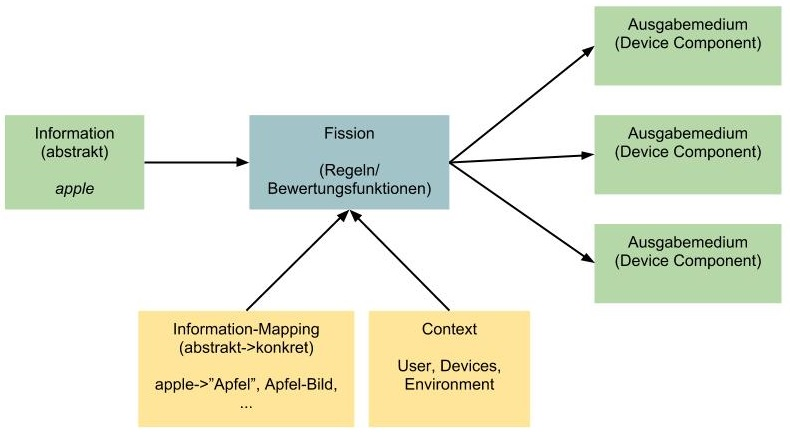
\includegraphics[width=.8\textwidth]{images/FissionUebersicht}
    \caption{\label{fission}Vereinfachte Übersicht der Funktionsweise der Fission}
\end{figure}
Dies läuft im Moment wie folgt ab: Abstrakte Informationen werden vom Dialog-Manager an die Fission gesendet. Diese abstrakten Informationen werden dann von der Fission wie in Abbildung \ref{fission} zu sehen verarbeitet. Die Fission legt mittels eines Information-Mappings fest, wie die abstrakten Informationen als konkrete Informationen dargestellt werden können. So könnte zum Beispiel die abstrakte Information \emph{apple} sowohl als Text als auch als Bild dargestellt werden. Diese konkreten Daten werden dann im Bezug auf die vorhandenen Kontextinformationen (wie  User-, Environment- oder Device-Context bewertet.
Diese Bewertung erfolgt mit sogenannten Regeln bzw. Bewertungsfunktionen\todor{Ich denke die genaue Definition  wäre dann Teil der Bachelorarbeit?}. Eine solche Regel besteht dabei aus einem Regel-Rumpf\todor{Ist Regel-Rumpf als Begriff okay? Sollte hier vllt eine echte Regel (z.B. Code Snippet) abgebildet werden?}, z.B. \glqq Es ist sehr gut den akustischen Kanal einzusetzen wenn der Nutzer blind ist\grqq. Außerdem besitzt jede Regel einen Funktionswert, der positiv oder negativ sein kann. Alle Regeln werden dann auf alle Kombinationen aus konkreten Informationen und Ausgabemedien(Devices) angewendet. Dabei kann jede Regel mit einer unterschiedlichen Gewichtung in die Bewertung einfließen. Die Gewichtung geht aus dem Kontext hervor.
\linebreak
Dieser Ansatz der Bewertung hat vermutlich exponentielle Laufzeitkomplexität. Davon ausgehend, dass bereits ein weitestgehend optimaler Algorithmus genutzt wird um die Bewertung der Regeln zu berechnen soll dieser Ansatz nun evaluiert werden. Dies dient dazu Aussagen über den Einfluss der Variablen auf die Laufzeit treffen zu können. 


\section{Geplantes Vorgehen}
Das Vorgehen kann in drei Teile, die Analyse, Evaluation und Bewertung des aktuellen Ansatz aufgeteilt werden. Ziel ist es klare Aussagen über das Laufzeitverhalten der Fission bei sich ändernden Variablen (siehe hierzu auch Evaluation) zu treffen.

\subsection{Analyse}
Hierbei geht es um eine theoretische Betrachtung des aktuell gewählten Ansatzes. Es soll z.B. der Algorithmus klassifiziert und seine theoretische Laufzeitkomplexität bestimmt werden. Auf Basis dieser Analyse werden dann bei der Evaluation zu prüfende Werte/Grenzen festgelegt, die der Algorithmus einhalten soll(te). Es sollten außerdem für die Evaluation nötigen Kriterien, Regeln und Kontexte definiert werden die dann wiederum wichtigen Einfluss auf die Planung haben.

\subsection{Evaluation}
Zur Evaluation soll ein Tool entwickelt werden, welches den Bewertungsalgorithmus der Fission unabhängig testen kann, dabei soll es möglich sein alle Variablen verändern zu können: Abstrakte Daten, Daten-Mappings, Kontext (User, Environment, Device). Außerdem muss das Evaluations-Tool in der Lage sein die Laufzeiten zu erfassen und angemessen zu protokollieren. Zur Implementierung des Evaluations-Tools ist sowohl ein Entwurf als auch anschließender Test nötig\todor{Muss hierauf genauer eingegangen werden? Ist ja das Arbeitspaket mit dem größten Zeitaufwand}. Die genauen Anforderungen an das Evaluations-Tool gehen aus der Analyse hervor. Diese Ergebnisse sind Grundlage für die Planung der Test-Settings. Diese sollen dann durchlaufen und deren Laufzeiten protokolliert werden.


\subsection{Auswertung}
Im Anhschluss an die Evaluation sollen die daraus resultierenden Ergebnisse bewertet werden. Ziel ist es Richt- bzw. Grenzwerte für die maximale Anzahl an Variablen die den Bewertungsalgorithmus der Fission beeinflussen zu empfehlen\todor{Das ist doch das Hauptziel, richtig? :)}.
Eventuell kann aus den Ergebnissen und der Analyse auch eine Anpassung \todor{Eventuell... schreibt man das ins Exposé rein oder hat man das halt im Hinterkopf?} des Algorithmus empfohlen werden.


\section{Geplante Gliederung}
\begin{itemize}
    \item  Motivation
    \item  Beschreibung der Problemstellung
    \begin{itemize}
        \item  Regeln/Evaluationsfunktionen
        \item  Kontext
        \item  Abstrakte Informationen
        \item  Informationsmapping
        \item  Ausgabemedien (Device components)
    \end{itemize}
    \item  Analyse
    \begin{itemize}
        \item  Beschreibung des aktuellen Ansatz (Algorithmus)
        \item  Theoretische Bewertung
        \item  Evtl. Vergleich mit ähnlichen Lösungen
    \end{itemize}
    \item  Evaluation
    \begin{itemize}
        \item  Planung
        \item  Entwicklung Evaluationstool
        \item  Durchführung
    \end{itemize}
    \item  Auswertung
     \begin{itemize}
     	\item  Zusammenfassung
     	\item  Diskussion
        \item  Evtl. Verbesserungsansätze
    \end{itemize}
\end{itemize}


\section{Zeitabschätzung}
Bei einer Bachelorarbeit im Umfang von 12 LP können 40 Tage für die eigentliche Durchführung geplant werden. Aus der Gliederung ergibt sich also folgende Zeitabschätzung\todor{Zu grob?}:
\begin{table}[h]
    \centering
    \begin{tabular}{|l|l|l|}
    	\hline
        Arbeitspaket & Zeit in Tagen \\
        \hline
        Beschreibung der Problemstellung & 2 Tage \\
        Analyse & 5 Tage \\
        Evaluation - Planung & 5 Tage \\
        Evaluation - Entwicklung Evaluationstool & 12 Tage \\
        Evaluation - Durchführung & 5 Tage \\
        Auswertung - Zusammenfassung & 2 Tage \\
        Auswertung - Diskussion & 4 Tage \\
        Auswertung - Evtl. Verbesserungsansätze & 5 Tage \\
        \hline
        Gesamt & 40 Tage \\
        \hline
        
    \end{tabular}
\end{table}

\todor{Letzter Punkt einplanen oder lieber Pufferzeit?}

% hier weitere Kapitel einbinden


%%
%% Anhänge
%%
%%\appendix
%%\chapter{Quelltexte}

In diesem Anhang sind einige wichtige Quelltexte aufgeführt.

\begin{lstlisting}
public class Hello {
    public static void main(String[] args) {
        System.out.println("Hello World");
    }
}
\end{lstlisting}



%%
%% Nachspann
%%
%%\backmatter


%%
%% Literaturverzeichnis
%%
%%\bibliography{bibliography}


%%
%% Versicherung
%%
%%\cleardoublepage
%%\thispagestyle{empty}

%%Name: \fullname \hfill Matrikelnummer: \matnr \vspace{2cm}

%%\minisec{Erklärung}

%%Ich erkläre, dass ich die Arbeit selbständig verfasst und keine anderen als die angegebenen Quellen und Hilfsmittel verwendet habe.\vspace{2cm}

%%Ulm, den \dotfill

%%\hfill {\footnotesize \fullname}
\end{document}
